\section{Planning}
\label{sec::planning}
All rooms in the map must be checked in order to find cups. The robot must be within 2 meters of a cup in order to actually detect the cup and within 1 meter in order to collect it. Cups are marked in the map using one pixel with grayscale value 150. Cups can be unloaded at the two offloading stations in the cafeteria. The offloading stations are represented with pixel values 100. The robot must start and end at an offloading station.\\[0.2cm]
You are free in regard in choice of algorithms. However, please document what algorithm you choose, how many kilometers the robot moves and how long it takes to calculate the path the robot takes.\\[0.2cm]
All planning is done offline, and it involves the functions:
\begin{itemize}\itemsep-2pt
\item \textbf{Wavefront} from the two unloading--stations
\item \textbf{Detection} of the rooms and blocks
\item \textbf{Priority queues} for each block and the
\end{itemize}

\subsection{Solution}
The first thing that happens in the planning part, is that a wavefront is generated from the two positions where the unloading--stations are located in the cafeteria. Cups are also seen as obstacles, when the wavefront is generated. The pixel values for the two unloadings stations are 
\begin{eqnarray*}
Unloading-station\: 1&:& \hspace{1cm}(3100,1400) \\
Unloading-station\: 2&:& \hspace{1cm}(2150,1400) \\
\end{eqnarray*}
and figure \ref{fig::path} shows how the wavefront expands from the two unloading--stations in the complete map. The unloading stations are the two darkest areas on the figure.\\[.2cm]
The wavefront--values is stored in a 2D--array, so when it is time for emptying the container, it is possible run the wavefront--function quickly in the online part. The generated array takes up some memory, but it saves time keeping the wavefront--map to the two unloading stations. When the cup container is filled, a path to the nearest unloading--station is found by using the offline wavefront function, \lstinline|makeWaveFrontoffline(currentX,currentY)|. For each pixel the robot moves through the wavefront path to a station, each coordinate is pushed into a vector--pair, so it can take the same path back to where it were interrupted by popping the values from the vector--pair. Just like Hansel and Gretel with the breadcrumbs, except that the robot will not get lost in the woods, find a gingerbread house, be fattened and so on.  

\begin{figure}[H]
\centering
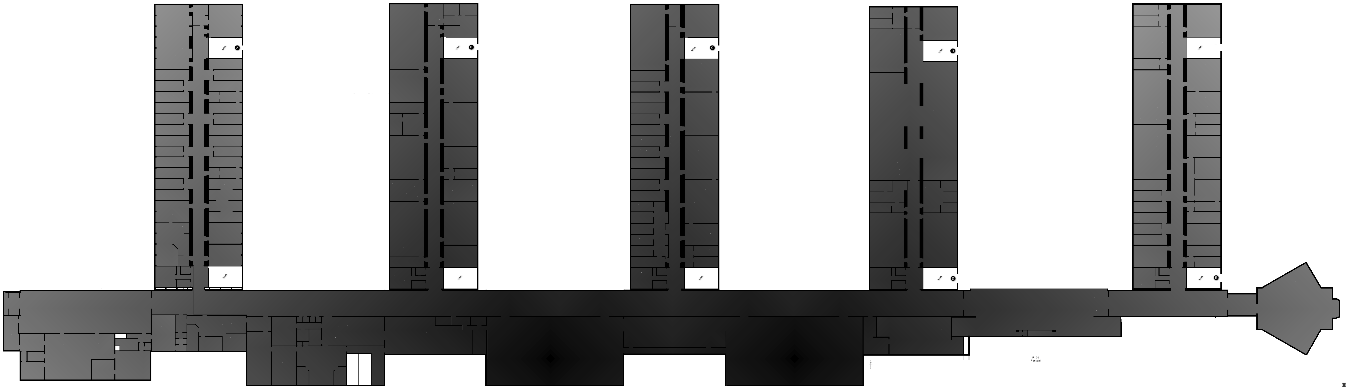
\includegraphics[scale=0.33]{img/wavefront_path.png}
\caption{How the wavefront expands from the two unloading--stations in the complete map.}
\label{fig::path}
\end{figure}

Detection of a room has four steps
\begin{enumerate}\itemsep-3pt
\item First the upper left corners ($C_{ul}$) of the squares are detected. Each pixel in the map is checked with a 3x3--mask, shown in table \ref{tab::ul_mask}, which looks at if the pixel value neighbors are obstacles, which corresponds to a left corner. If the mask matches, then the pixel is marked as a $C_{ul}$ and the position for the pixel is stored in a data type, called \lstinline|square|. 

\begin{table}[H]
\centering
\begin{tabular}{|l|l|l|}
\hline
0 & 0 & 0 \\ \hline
0 & P &   \\ \hline
0 &   &   \\ \hline
\end{tabular}
\caption{3x3 mask for detecting upper left corners}
\label{tab::ul_mask}
\end{table}

\item Next the upper right corners ($C_{ur}$) is found by taking the the position for each $C_{ul}$, and then keep moving to the right, until it hits an obstacle. When it hits an obstacle, the pixel just before is marked as a $C_{ur}$ and stored in \lstinline|square|. On table \ref{tab::corner_detection} is this approach shown.
\item Next the lower left corners $C_{ll}$ is found, just like the $C_{ur}$, by taking the the position for each $C_{ul}$, but instead it keeps moving down, until it hits an obstacle. When it hits an obstacle, the pixel just before is marked as a $C_{ll}$ and stored in \lstinline|square|. On table \ref{tab::corner_detection} is this approach shown. 
\item The lower right corner ($C_{lr}$) is not detected like the other three corners, it is calculated by taking the height distance (in pixels) between $C_{ul}$ and $C_{ll}$, and assuming that the $C_{lr}$ has the same height distance from the $C_{ur}$. Like the other corners, the $C_{lr}$ is marked and stored in \lstinline|square|. 
\end{enumerate} 

\begin{table}[H]
\centering
\begin{tabular}{|c|
>{\columncolor[HTML]{C0C0C0}}c ccccccc|c|}
\hline
\cellcolor[HTML]{000000}{\color[HTML]{FFFFFF} 0} & \multicolumn{1}{l|}{\cellcolor[HTML]{000000}{\color[HTML]{FFFFFF} 0}} & \multicolumn{1}{l|}{\cellcolor[HTML]{000000}{\color[HTML]{FFFFFF} 0}} & \multicolumn{1}{l|}{}            & \multicolumn{1}{l|}{}            & \multicolumn{1}{l|}{}            & \multicolumn{1}{l|}{}            & \multicolumn{1}{l|}{}            &                                  &                                                  \\ \hline
\cellcolor[HTML]{000000}{\color[HTML]{FFFFFF} 0} & \cellcolor[HTML]{9B9B9B}$C_{ul}$                                      & \cellcolor[HTML]{C0C0C0}$\cdots$                                      & \cellcolor[HTML]{C0C0C0}$\cdots$ & \cellcolor[HTML]{C0C0C0}$\cdots$ & \cellcolor[HTML]{C0C0C0}$\cdots$ & \cellcolor[HTML]{C0C0C0}$\cdots$ & \cellcolor[HTML]{C0C0C0}$\cdots$ & \cellcolor[HTML]{9B9B9B}$C_{ur}$ & \cellcolor[HTML]{000000}{\color[HTML]{FFFFFF} 0} \\ \cline{1-1} \cline{10-10} 
\cellcolor[HTML]{000000}{\color[HTML]{FFFFFF} 0} & $\vdots$                                                              & \cellcolor[HTML]{C0C0C0}                                              & \cellcolor[HTML]{C0C0C0}         & \cellcolor[HTML]{C0C0C0}         & \cellcolor[HTML]{C0C0C0}         & \cellcolor[HTML]{C0C0C0}         & \cellcolor[HTML]{C0C0C0}         & \cellcolor[HTML]{C0C0C0}$\vdots$ &                                                  \\ \cline{1-1} \cline{10-10} 
                                                 & $\vdots$                                                              & \cellcolor[HTML]{C0C0C0}                                              & \cellcolor[HTML]{C0C0C0}         & \cellcolor[HTML]{C0C0C0}         & \cellcolor[HTML]{C0C0C0}         & \cellcolor[HTML]{C0C0C0}         & \cellcolor[HTML]{C0C0C0}         & \cellcolor[HTML]{C0C0C0}$\vdots$ &                                                  \\ \cline{1-1} \cline{10-10} 
                                                 & \cellcolor[HTML]{9B9B9B}$C_{ll}$                                      & \cellcolor[HTML]{C0C0C0}$\cdots$                                      & \cellcolor[HTML]{C0C0C0}$\cdots$ & \cellcolor[HTML]{C0C0C0}$\cdots$ & \cellcolor[HTML]{C0C0C0}$\cdots$ & \cellcolor[HTML]{C0C0C0}$\cdots$ & \cellcolor[HTML]{C0C0C0}$\cdots$ & \cellcolor[HTML]{9B9B9B}$C_{lr}$ &                                                  \\ \hline
                                                 & \multicolumn{1}{l|}{\cellcolor[HTML]{000000}{\color[HTML]{FFFFFF} 0}} & \multicolumn{1}{l|}{}                                                 & \multicolumn{1}{l|}{}            & \multicolumn{1}{l|}{}            & \multicolumn{1}{l|}{}            & \multicolumn{1}{l|}{}            & \multicolumn{1}{l|}{}            &                                  &                                                  \\ \hline
\end{tabular}
\caption{Detection of the room corners}
\label{tab::corner_detection}
\end{table}

When all the rooms are detected, the center of each room is calculated, by taking the half of the weight and height of the room, and stores it as a vector--pair. Each room in the list is then check wherever a room is actually a room or a hallway by looking at the relationship between the wall of the room. Some thresholds are set, so if the relationship excites these threshold, then the room is detected as a hallway instead. On figure \ref{fig::graph} can it be seen how the different rooms are connected to each hallway. The hallways has a priority queue, which prioritizes the room after the distance between the center of the hallway to the center of the room. Each room is put in the priority queue of that hallway center that is closest to the center of the room. This priority for each hallway is the order of which room that are cleaned and emptied for cups first.

\begin{figure}[H]
\centering
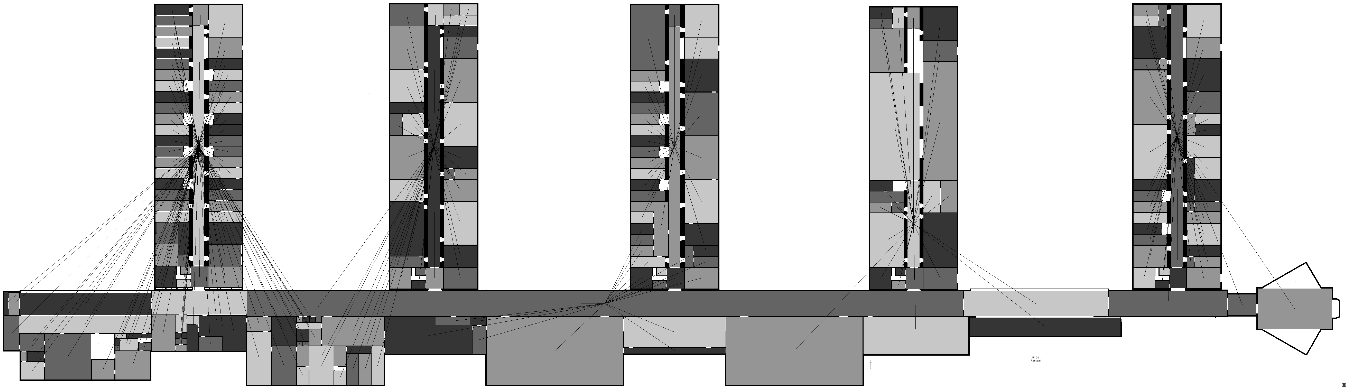
\includegraphics[scale=0.33]{img/graph.png}
\caption{An overview of how the different rooms are detected and connected to each hallway on the complete map of SDU.}
\label{fig::graph}
\end{figure}

\subsection{Results}